

\documentclass{beamer}
 
\usepackage[utf8]{inputenc}
 \usetheme{Madrid}
 \usecolortheme{beaver}
 \usefonttheme{structuresmallcapsserif}
 \usepackage{listings}
%Information to be included in the title page:


\title[Distributed Systems] %optional
{Communication}

\subtitle{An Overview}

\author[Dr. Joseph Kehoe] % (optional, for multiple authors)
{Joseph Kehoe\inst{1}}

\institute[IT Carlow] % (optional)
{
	\inst{1}%
	Department of Computing and Networking\\
	Institute of Technology Carlow
}

\date[ITC 2018] % (optional)
{CDD101, 2018}

\logo{
\includegraphics[height=1.5cm]{../../itcarlowlogo.png}}




 
 \AtBeginSection[]
 {
 	\begin{frame}
 		\frametitle{Table of Contents}
 		\tableofcontents[currentsection]
 	\end{frame}
 }
 
 
 
\begin{document}
 
\frame{\titlepage}
 
  \begin{frame}
  	\frametitle{Table of Contents}
  	\tableofcontents
  \end{frame}
 

\section{Overview}
  \begin{frame}
  	\frametitle{Communication Overview}
  	Computers in a distributed system may have different:
  	\begin{itemize}
  		\item Architectures
  		\item Operating Systems
  		\item Data encoding
  		\item programming languages
  	\end{itemize}
We need a system of communication that allows them to talk to each other transparantly
  	
  		%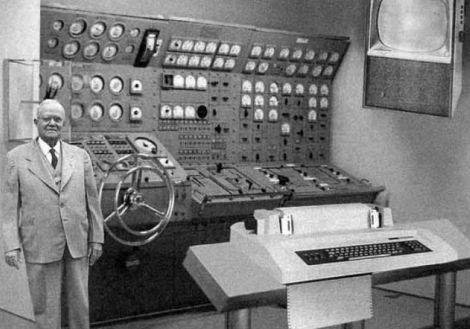
\includegraphics[height=4cm]{Old-Server.jpg}
  \end{frame}
  
\section{Protocols}

  \begin{frame}
  	\frametitle{Networking Protocols}
  	Communication between computers is build on existing network protocols
  	\begin{itemize}
  		\item At the base we have TCP/IP or UDP/IP
  		\item We can use socket programming to use these directly
  		\item Or we can use higher level protocols instead of or alongside this: e.g. HTTP
  		\item This base level protocol is available to all computers
  		\item But we will need to add a layer on top of this base in order to give us the extra features we need
  	\end{itemize}
I am going to assume you are familiar with these lower level protocols
  	
  	%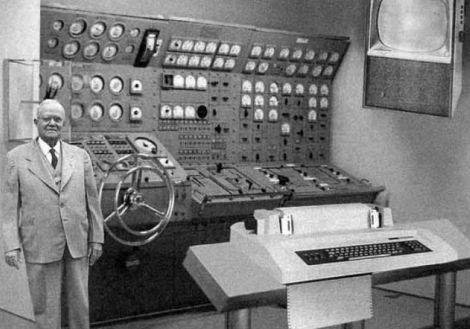
\includegraphics[height=4cm]{Old-Server.jpg}
  \end{frame}

\section{Remote Procedure Call}
  \begin{frame}
  	\frametitle{RPC}
  	Allow code to call procedures not resident on the local machine
  	\begin{itemize}
  		\item Causes a procedure to execute in a different address space (commonly on another computer on a shared network), which is coded as if it were a normal (local) procedure call, without the programmer explicitly coding the details for the remote interaction. 
  		\item The programmer writes essentially the same code whether the subroutine is local or remote
  		\item Suited to Client Server Architectures
  		\item RPC is a form of Inter Process Communication (IPC)
  		\item RPC is usually synchronous in nature
  	\end{itemize}
  	%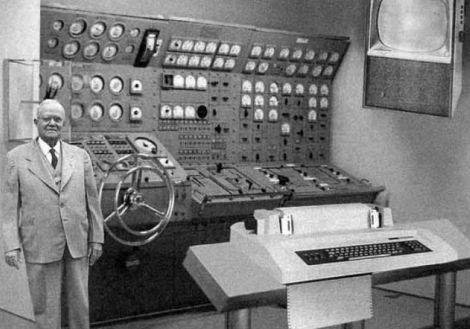
\includegraphics[height=4cm]{Old-Server.jpg}
  \end{frame}
  
  
  
  
    	
 \begin{frame}
 	\frametitle{RPC}
 	Sequence of events
 	\begin{itemize}   	
	   \item The client calls the client stub. The call is a local procedure call, with parameters pushed on to the stack in the normal way.
    	\item The client stub packs the parameters into a message and makes a system call to send the message. Packing the parameters is called marshalling.
    	\item The client's local operating system sends the message from the client machine to the server machine.
    	\item The local operating system on the server machine passes the incoming packets to the server stub.
    	\item The server stub unpacks the parameters from the message. Unpacking the parameters is called unmarshalling.
    	\item Finally, the server stub calls the server procedure. The reply traces the same steps in the reverse direction.
   	\end{itemize}
   	%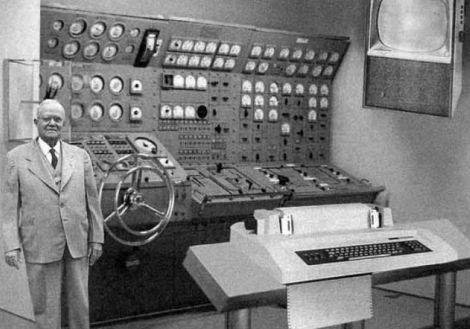
\includegraphics[height=4cm]{Old-Server.jpg}
   \end{frame} 
   \begin{frame}
   	\frametitle{IDL}
   	To let different clients access servers, a number of standardized RPC systems have been created.
   	\begin{itemize}
        \item Most of these use an interface description language (IDL) to let various platforms call the RPC
        \item The IDL files can then be used to generate code to interface between the client and servers.
    \end{itemize}
    \begin{itemize}
	    \item XML-RPC is an RPC protocol that uses XML to encode its calls and HTTP as a transport mechanism.
	    \item JSON-RPC is an RPC protocol that uses JSON-encoded messages
	    \item JSON-WSP is an RPC protocol that uses JSON-encoded messages
	    \item SOAP is a successor of XML-RPC and also uses XML to encode its HTTP-based calls.
    \end{itemize}
     	%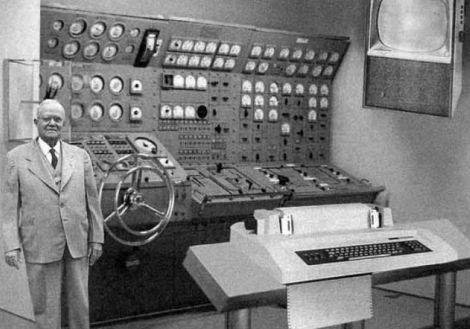
\includegraphics[height=4cm]{Old-Server.jpg}
     \end{frame} 
     
     \begin{frame}
     	\frametitle{RPC}
     	
     	\begin{itemize}
     		\item Packaging of parameters for transport to remote server is called \textbf{Marshalling}
     		\item Parameters are either:
     		\begin{itemize}
     			\item Pass by Value
     			\item Pass by Reference
     			\item Pass by copy Restore
     		\end{itemize}
     		\item Passing pointers is obviously very difficult
     	\end{itemize}
     	     	%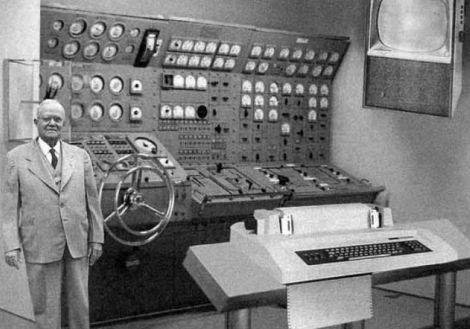
\includegraphics[height=4cm]{Old-Server.jpg}
     \end{frame}
  
\section{Remote Object Invocation}

   \begin{frame}
   	\frametitle{ROI}
   	
   	\begin{itemize}
   		\item Extends RPC to objects
   		\item Improves on RPC
   		\item Objects seperate state from interface (perfect for distributed Objects!)
   		\item Keep state on server and put Interface on client
   		\item Local proxy implements interface and holds reference to remote object
   		\item It marshals data before sending, sends data, receives return values and unmarshalls them 
   	\end{itemize}
   	%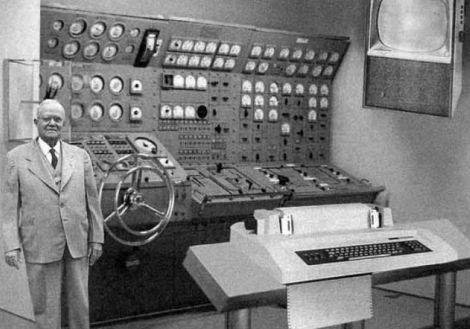
\includegraphics[height=4cm]{Old-Server.jpg}
   \end{frame}
   
      \begin{frame}
      	\frametitle{ROI (on server)}
      	
      	\begin{itemize}
      		\item Server has a server "stub" known as a skeleton
      		\item This receives data, unmarshals it and calls the server object implementation. It then marshalls the return values and sends them back to the client proxy
      		\item Often use the \textbf{Object Adapter} pattern to wrap an object interface around an existing system
      		\item Object is transient if it cannot be offloaded from server. So if server goes down object is lost
      	\end{itemize}
      	%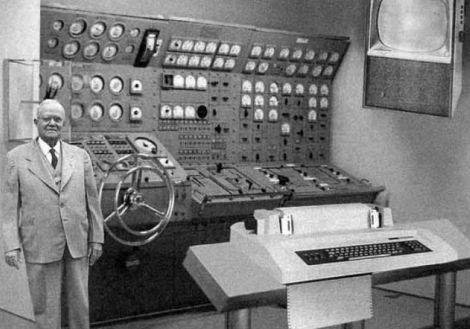
\includegraphics[height=4cm]{Old-Server.jpg}
      \end{frame}
      
            \begin{frame}
            	\frametitle{ROI (Objecct References)}
            	\begin{itemize}
            		\item Object is persistent if it can be offloaded (saved) from the server to backup storage. 
            		\item This allows the object to be reanimated if the server crashes
            		\item This even allows us to move the object around if we have a system wide object reference
            		\item Need a DNS for object references if this is to work.
            	\end{itemize}
            	%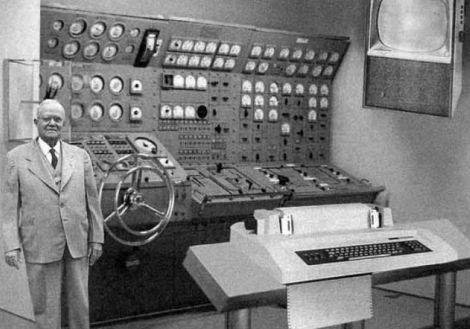
\includegraphics[height=4cm]{Old-Server.jpg}
            \end{frame}
      \begin{frame}
      	\frametitle{ROI (Dynamic Invocation)}
      	\begin{itemize}
      		\item If IDL is compiled at runtime then we have\textbf{ Static Object Invocation}
      		\item If we can decode interface at runtime then we have \textbf{Dynamic Object Invocation}
      		\item Static Call is:  accountRef->deposit(500);
      		\item Dynamic Call is: sendMessage(accountRef,deposit,500)
      	\end{itemize}
      	%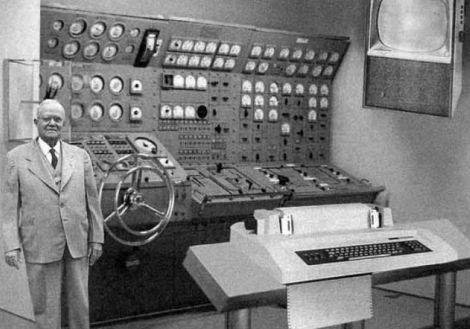
\includegraphics[height=4cm]{Old-Server.jpg}
      \end{frame}      
      \begin{frame}
      	\frametitle{ROI (efficiency)}
      	\begin{itemize}
      		\item Remote Object Innvocation can be inefficient
      		\item Esp. if object state is small or parameters are large
      		\item If system can distinguish between local and remote objects then we can circumvent this
      	\end{itemize}
      	%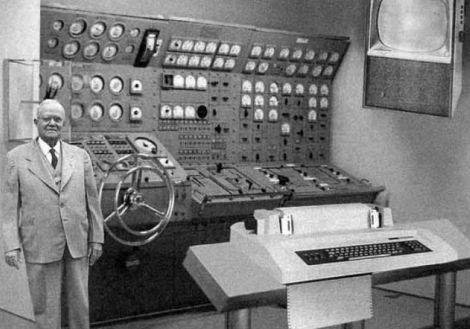
\includegraphics[height=4cm]{Old-Server.jpg}
      \end{frame}  
      \begin{frame}
      	\frametitle{Java RMI}
      	\begin{itemize}
      		\item Integrated into the language (high level approach)
      		\item Cloning of remote objects is difficult so local proxy is not cloned during process, just the remote obejct
      		\item We must explicitly get a new reference to the remote cloned object
      		\item Remote objects cannot be \textbf{synchronised} - only the proxy can be
      		\item Why? hint: Client crashes during operation
      		\item Anything serialisable can be marshalled
      		\item Proxys can be serialised (so we can pass them around)
      	\end{itemize}
      	%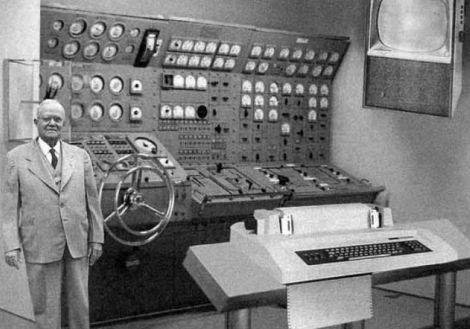
\includegraphics[height=4cm]{Old-Server.jpg}
      \end{frame}          
\section{Messaging}

\end{document}

